%% intro.tex
%%
%% Copyright 2017 Evandro Coan
%% Copyright 2012-2016 by abnTeX2 group at http://www.abntex.net.br/
%%
%% This work may be distributed and/or modified under the
%% conditions of the LaTeX Project Public License, either version 1.3
%% of this license or (at your option) any later version.
%% The latest version of this license is in
%%   http://www.latex-project.org/lppl.txt
%% and version 1.3 or later is part of all distributions of LaTeX
%% version 2005/12/01 or later.
%%
%% This work has the LPPL maintenance status `maintained'.
%% The Current Maintainer of this work is the Evandro Coan.
%%
%% The last Maintainer of this work was the abnTeX2 team, led
%% by Lauro César Araujo. Further information are available on
%% https://www.abntex.net.br/
%%
%% This work consists of a bunch of files. But originally there ware 3 files
%% which are renamed as follows:
%% Renamed the `abntex2-modelo-include-comandos` to `chapters/chapter_01.tex`
%% Renamed the `abntex2-modelo-trabalho-academico.tex` to `chapters/intro.tex`
%% Renamed the `abntex2-modelo-references.bib` to `aftertext/modelo-ufsc-references.bib`
%%
%% This file was originally the main template file, however this main file was
%% split into several new files, which are respectively drastically changed,
%% except this files which contains most of the main documentation message.
%%

% ------------------------------------------------------------------------
% ------------------------------------------------------------------------
% abnTeX2: Modelo de Trabalho Academico (tese de doutorado, dissertacao de
% mestrado e trabalhos monograficos em geral) em conformidade com
% ABNT NBR 14724:2011: Informacao e documentacao - Trabalhos academicos -
% Apresentacao
% ------------------------------------------------------------------------
% ------------------------------------------------------------------------

% The \phantomsection command is needed to create a link to a place in the document that is not a
% figure, equation, table, section, subsection, chapter, etc.
% https://tex.stackexchange.com/questions/44088/when-do-i-need-to-invoke-phantomsection
\phantomsection

% https://tex.stackexchange.com/questions/5076/is-it-possible-to-keep-my-translation-together-with-original-text
\chapter{\lang{Introduction}{Introdução}}
\phantomsection

A Tabela~\ref{tab:a_table_formatacao_de_texto} mostra  informações do modelo de teses da Biblioteca Universitária da UFSC (BU-UFSC).

% What does [t] and [ht] mean?
% https://tex.stackexchange.com/questions/8652/what-does-t-and-ht-mean
%
% How can I get rid of the LaTeX warning: Float too large for page?
% https://tex.stackexchange.com/questions/36252/how-can-i-get-rid-of-the-latex-warning-float-too-large-for-page
%
% "warning: Text page X contains only floats" How to suppress this warning?
% https://tex.stackexchange.com/questions/223149/warning-text-page-x-contains-only-floats-how-to-suppress-this-warning
%
% Make a table span multiple pages
% https://tex.stackexchange.com/questions/26462/make-a-table-span-multiple-pages
%
% How to make the longtable to work with centering & caption on memoir class?
% https://tex.stackexchange.com/questions/386541/how-to-make-the-longtable-to-work-with-centering-caption-on-memoir-class
%
% How to fix this Package array Error: Only one column-spec allowed?
% https://tex.stackexchange.com/questions/367069/how-to-fix-this-package-array-error-only-one-column-spec-allowed
%
% How to auto adjust my last table column width, and why is there Underfull \vbox badness on this table?
% https://tex.stackexchange.com/questions/387238/how-to-auto-adjust-my-last-table-column-width-and-why-is-there-underfull-vbox/387251
\setlength\extrarowheight{2pt}
\begin{tabularx}{\linewidth}{>{\RaggedRight}p{3cm}|>{\arraybackslash}X}

    \caption[Formatação do texto]{Formatação do texto \showfont}
    \label{tab:a_table_formatacao_de_texto}                                                        \\
    \hline
    \endfirsthead

    % How to set font size of footnotes correctly in memoir?
    % https://tex.stackexchange.com/questions/213927/how-to-set-font-size-of-footnotes-correctly-in-memoir
    \multicolumn{2}{p{\dimexpr\textwidth-2\tabcolsep\relax}}{\ufsccaptionsize\tablename~\thetable:
        Formatação do texto (continuação) \showfont}                                               \\
    \hline
    \endhead

    % Set multicolumn width to default table width
    % https://tex.stackexchange.com/questions/99326/set-multicolumn-width-to-default-table-width
    \hline
    \multicolumn{2}{p{\dimexpr\textwidth-2\tabcolsep\relax}}{\footnotesize continua na próxima página\protect\englishword{\showfont}}
    \endfoot

    \hline
    \multicolumn{2}{p{\dimexpr\textwidth-2\tabcolsep\relax}}{\fonte{O autor -- \showfont} }
    \endlastfoot
    Cor                          & Branco - \englishword{\showfont}                                \\ \hline
    Formato do papel             & A4                                                              \\ \hline
    Gramatura                    & 75                                                              \\ \hline
    Impressão                    & Frente e verso                                                  \\ \hline
    Margens                      & Direita e superior 3, Inferior e esquerda: 2.                   \\ \hline
    Cabeçalho                    & 0,7                                                             \\ \hline
    Rodapé                       & 0,7                                                             \\ \hline
    Paginação                    & Externa                                                         \\ \hline
    Alinhamento vertical         & Superior                                                        \\ \hline
    Alinhamento do texto         & Justificado                                                     \\ \hline
    Fonte sugerida               & Times New Roman                                                 \\ \hline
    Tamanho da fonte             & 12 para o texto incluindo os títulos das seções e subseções.
    As citações com mais de três linhas as legendas das ilustrações
    e tabelas, fonte 10.                                                                           \\ \hline
    Espaçamento entre linhas     & Um e meio (1,5)                                                 \\ \hline
    Espaçamento entre parágrafos & Anterior 0,0; Posterior 0,0                                     \\ \hline
    Numeração da seção           & As seções  primárias devem  começar  sempre em páginas ímpares.
    Deixar um espaço (simples) entre o título da seção e o texto e
    entre o texto e o título da subseção.                                                          \\ \hline
\end{tabularx}


\begin{figure}
    \caption{Exemplo de figura}
    \label{fig:ex01}
    \centering
    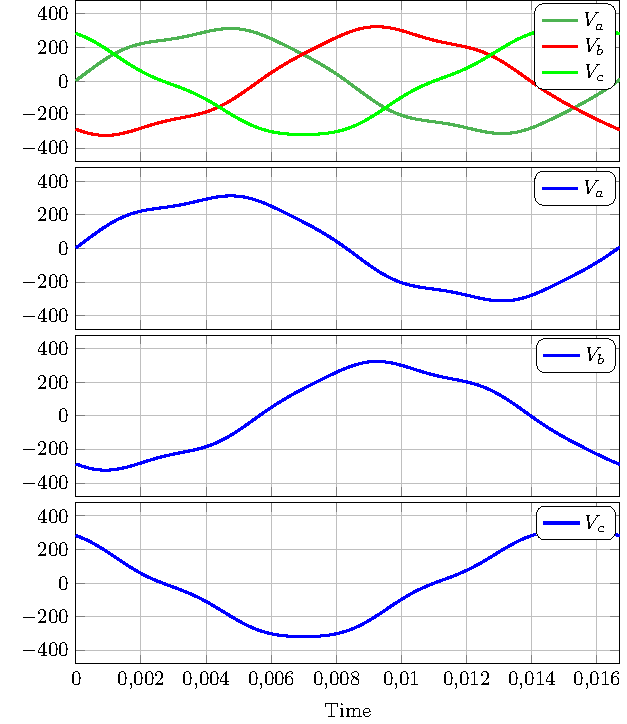
\includegraphics[width=\linewidth]{pictures/ex01}
    \fonte{o autor -- \showfont}
\end{figure}


Por exemplo, na \figref{fig:ex01}, tem-se...

\begin{figure}
    \caption{Exemplo de aquisição}
    \label{fig:tek0009}
    \centering
    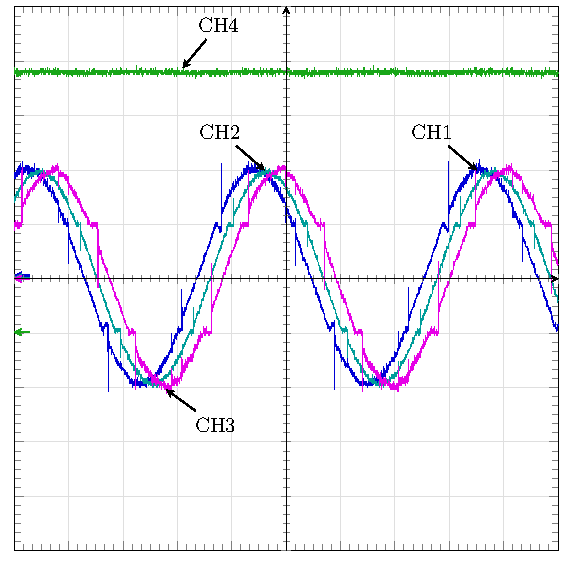
\includegraphics[width=0.9\linewidth]{pictures/tek0009}
    \fonte{o autor -- \showfont}
\end{figure}

Este documento e seu código-fonte são exemplos de referência de uso da classe
\textsf{abntex2} e do pacote \textsf{abntex2cite}. O documento
exemplifica a elaboração de trabalho acadêmico (tese, dissertação e outros do
gênero) produzido conforme a ABNT NBR 14724:2011 \emph{Informação e documentação
    - Trabalhos acadêmicos - Apresentação}.

A expressão ``Modelo Canônico'' é utilizada para indicar que \abnTeX{} não é
modelo específico de nenhuma universidade ou instituição, mas que implementa tão
somente os requisitos das normas da ABNT. Uma lista completa das normas
observadas pelo \abnTeX{} é apresentada em \textcite{abntex2classe}.

Sinta-se convidado a participar do projeto \abnTeX{}! Acesse o site do projeto em
\url{http://abntex2.googlecode.com/}. Também fique livre para conhecer,
estudar, alterar e redistribuir o trabalho do \abnTeX{}, desde que os arquivos
modificados tenham seus nomes alterados e que os créditos sejam dados aos
autores originais, nos termos da ``The \LaTeX{} Project Public
License''\footnote{\url{http://www.latex-project.org/lppl.txt}}.

Encorajamos que sejam realizadas customizações específicas deste exemplo para
universidades e outras instituições --- como capas, folha de aprovação, etc.
Porém, recomendamos que ao invés de se alterar diretamente os arquivos do
\abnTeX{}, distribua-se arquivos com as respectivas customizações.
Isso permite que futuras versões do \abnTeX{}~não se tornem automaticamente
incompatíveis com as customizações promovidas. Consulte
\textcite{abntex2-wiki-como-customizar} par mais informações.

Este documento deve ser utilizado como complemento dos manuais do \abnTeX{}
\cite{abntex2classe,abntex2cite,abntex2cite-alf} e da classe \textsf{memoir}
\cite{memoir}.

Esperamos, sinceramente, que o \abnTeX{} aprimore a qualidade do trabalho que
você produzirá, de modo que o principal esforço seja concentrado no principal:
na contribuição científica.

Equipe \abnTeX{}

Lauro César Araujo


